% (introduction)

% - overview (motivation, representation, types of carving; pipeline)
\section{Overview}  \label{method-overview}
Where space caving based on silhouettes (Structure from Silhouettes) has difficulties with high-textured environments and multi-view stereo techniques using depth maps have difficulties with low-textured or reflective environments, our method targets at scenes containing both. Specifically, it aims at reconstructing low-textured and reflective objects without relying on the ability to find \emph{any} features on the objects themselves - provided enough texture-rich surrounding objects are present. To get statistical reliable reconstructions, enough data needs to be provided; therefore, the proposed method works best with video footage shot while moving through the scene. The method is based on space carving and iteratively improves a model represented with a voxel grid. Carving is accomplished by shooting finite rays between camera poses and locations of triangulated features, affecting voxels hit by the ray segments only. This is different from photo-consistent space carving, which affects single voxels each step, and differs from silhouette-based space carving in the sense that carving stops at a specific point, allowing concavities to be reconstructed. Furthermore, the voxel grid is probabilistic, allowing confidence estimation for reconstructed three-dimensional structures depending on the amount of data used for each voxel.

Two algorithms are proposed based on visibility and occlusion information. Central to the taken approach is the intuition that the ability to see a feature with known location means it is unlikely that there exists an objects in between the observer and the feature, and not seeing an earlier seen feature means there could well be such an occluding object. The algorithms require as input calibrated cameras, a reliable feature cloud, and visibility lists describing which cameras successfully detecting which points. The input can be provided by standard Structure from Motion techniques. Output of the algorithms is a probabilistic (or thresholded) voxel grid representing occupancy probability, and can be used for further surface reconstruction if desired.

The first algorithm, called \textbf{Visibility Space Carving}, assumes all space is occupied by default, unless proven otherwise. Space between camera poses and corresponding detected features is then carved, that is, marked as free. In case the features are points without clear size (such as obtained by standard SfM), in practise means carving tubes the size of voxels. Output are those voxels which do re-project in at least one image plane, but for which could not be proven to not occlude anything, either due an actual occluder object or due to absence of information. 

The second algorithm, called \textbf{Visibility-Occlusion Space Carving}, starts with unknown occupancy state voxels. The occupancy probability is then altered by both visibility and occlusion information. Occupancy probability of voxels in space between camera poses and detected features is increased, and space between camera poses and undetected features is made more likely to be occupied. A slightly altered version is proposed for cases where visibility information is much more reliable than occlusion information, which can be caused by bad matches, as is often the case for publicly available SfM systems.

Collectively, the proposed algorithms could arguably be called \textbf{Structure from Visibility}. More detailed descriptions follow in Sections \ref{vis-carving} and \ref{vis-occ-carving}. For clarity reasons, a high-level overview of the complete pipeline from footage to reconstructed model is given next.


\subsection{Reconstruction pipeline}  \label{pipeline}

\begin{enumerate}
  \item \textbf{Shoot footage and extract images}
  \item \textbf{Structure from Motion} (Section \ref{sfm}) - Stable features (\ie SIFT) are found, matched over the sequence of images, and relative camera transformations are estimated. The features are triangulated and the resulting 3D feature clouds are combined (\ie Bundle Adjustment) to obtain global camera poses, features poses and visibility information of the features for all camera poses. Existing tools can be used for this step, which we review in Sect. \emph{implementation}.
  \item Optional: \textbf{Extend visibility lists} (Section \ref{extend-vis-lists}) - Many SfM systems are conservative with claiming visibility of features. It may help to review the visibility lists and attempting to extend them.
  \item \textbf{Space carving} (Sections \ref{vis-carving}-\ref{vis-occ-carving}) - Space is partitioned into a voxel grid. Using the camera poses, feature locations, and visibility information, the voxel grid is carved, obtaining occupancy probabilities for all voxels.
  % TODO: is this working?
  \item \textbf{Regularisation} (Section \ref{regularisation}) - The probabilistic voxel grid - containing independent voxels - is feed to a 3D graph cut algorithm to obtain a global solution where local smoothness is promoted.
  \item Optional: \textbf{Surface reconstruction} - Raw voxel grids can be processed further to obtain alternative surface representations such as a polygon mesh (\ie using Marching Cubes) or fitted surface (\ie Poisson Surface), followed by texture mapping. Surface reconstruction is well-established and will not be covered in this thesis. Our final result will be a voxel grid. % TODO or did we do it in the end?
  \item \textbf{Visualisation} (Section \ref{results}) - Depending on the final representation, results can be displayed in a appropriate way. They can be rendered from original camera poses, or new positions. They can be rendered as 3D voxel grid, depth map, annotated on original images (original poses only) or texture-mapped (useful for new poses). Being able to interact with a 3D model usually greatly improves the ability to estimate geometry.
\end{enumerate}


% - visibility carving
\pagebreak
\section{Visibility Space Carving}  \label{vis-carving}

\begin{figure}[htb!]
 \centering
 \subfigure[Probabilistic visibility track / list (curved blue plot) over image sequence for one interest point (blue arrow)]{
  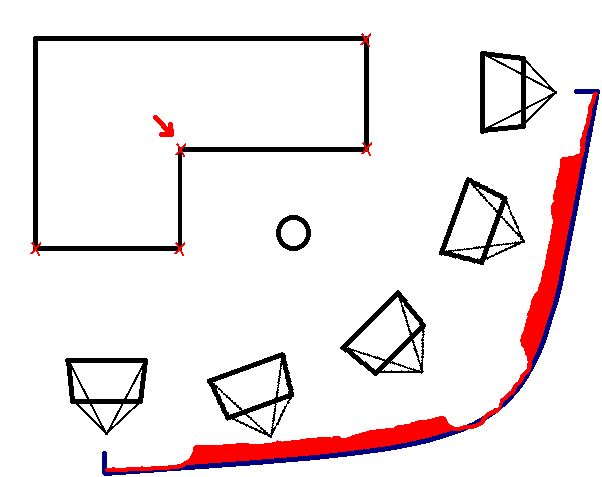
\includegraphics[width=0.45\textwidth]{img/visibilitytrack}
  \label{fig:visibilitytrack}
 }
 \subfigure[Carving away space based on one visibility track]{
  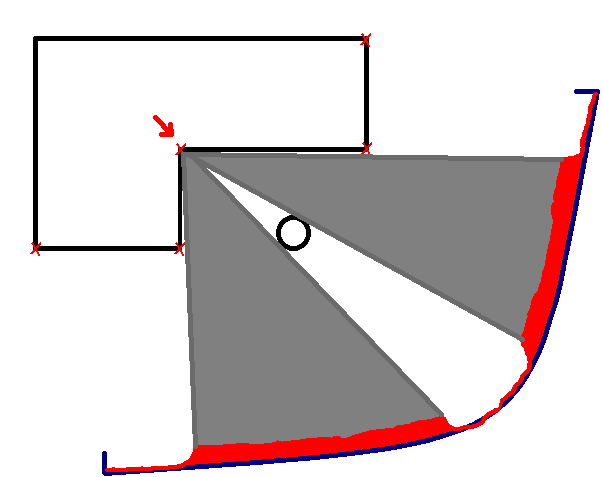
\includegraphics[width=0.45\textwidth]{img/visibilitycarving}
          \label{fig:visibilitycarving}
 }
 \caption{Graphical example of Visibility Space Carving. Cameras in (a) represent a dense sequence of camera poses, hence the `interpolation' in between.}
 \label{fig:vis-carving}
\end{figure}

{\singlespacing
\begin{algorithm}[!h]
  \centering
  \begin{algorithmic}[1]
    \Function{VisibilitySpaceCarving}{$c$, $f$, $v$, $r$} \Comment{Arguments: cameras $c$, features $f$, visibility lists $v$, voxel grid resolution $r$}
      \State $G \gets G_{'unknown'}(r)$ \Comment{Initialise voxel grid $G$ with label `unknown' and finite size}
      \ForAll{Feature $f_i$ in $f$}
        \ForAll{Camera $c_j$ in $v_{f_i}$} \Comment{Get all camera poses that detected this feature}
          \State $X \gets \mathrm{getVoxelsBetween}(G, c_j, f_i)$ \Comment{Get voxels in between camera and feature}
          \ForAll{Voxel $x_i$ in $X$}
            \State $x_i \gets \mathrm{free}$ \Comment{Mark voxel as `free'}
          \EndFor
        \EndFor
      \EndFor
      \State $H \gets H_{'free'}(r)$ \Comment{Initialise voxel grid $H$ with label `free' and same indexes as $G$}
      \ForAll{Voxel $G_i$ in $G$}
        \State $visible \gets \mathrm{false}$
        \ForAll{Camera $c_j$ in $c$}
          \If{$\mathrm{reprojectsInsideImage}(G_i, c_j)$}
            \State $visible \gets \mathrm{true}$
          \EndIf
        \EndFor
        \If{$visible$}
          \State $H_i \gets G_i$ \Comment{Only export the state of those voxels that could have been visible}
        \EndIf
      \EndFor
      \State \Return $H$
    \EndFunction
  \end{algorithmic}
  \caption{Visibility Space Carving}
  \label{alg:vis-carving}
\end{algorithm}
}

The Visibility Space Carving algorithm has its origins in Space Carving based on Silhouettes. It starts with a fully occluded world-view and carves away space that is not occluded. It does not carve space based on silhouettes until infinity, but carves until visible triangulated features (\ie SIFT interest points). Voxels between camera poses and features are found (\ie by shooting rays) and set to free. Since this is a binary process, the algorithm uses two labels instead of probabilities. The process for one interest point is shown in Figure \ref{fig:vis-carving}. Note that Structure from Motion can give an indication of the chance a feature is present (\ie how good the match is), but here we use thresholded, binary visibility lists and standard SfM tools often export only these. Also note that the example is shown in 2D and one interest point will only carve away one slice of space. If enough features are used, space will be carved away in a substantial part of the free space in the scene. After the carving step, a subspace of the grid is exported as output. Since voxels outside the camera views will always be occluded, we project the voxels onto the camera planes and export only those that project on at least one camera window. The algorithm is described more formally in Alg.~\ref{alg:vis-carving}.

% - visibility and occlusion carving (general version, absolute vote / stable points version)
%\pagebreak
\section{Visibility-Occlusion Space Carving}  \label{vis-occ-carving}

\begin{figure}[htb!]
 \centering
 \subfigure[Probabilistic visibility track / list (curved blue plot) over image sequence for one interest point (blue arrow)]{
  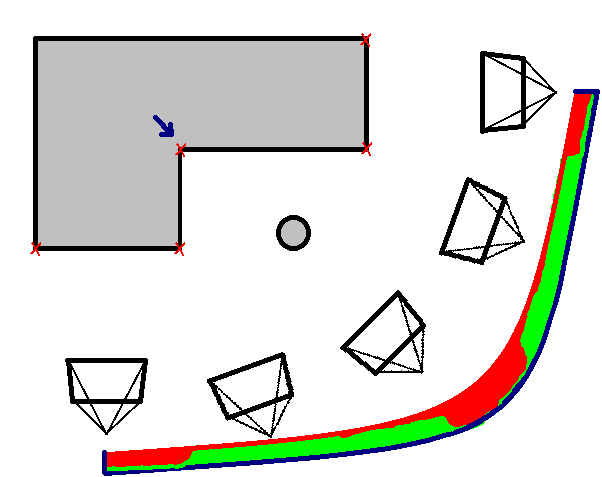
\includegraphics[width=0.45\textwidth]{img/visibilityocclusiontrack}
  \label{fig:visibilitytrack}
 }
 \subfigure[Increasing (green) or decreasing (red) occupancy probability based on one visibility track. Space that is likely to get high occupancy probabilities after processing all data are coloured darker red.]{
  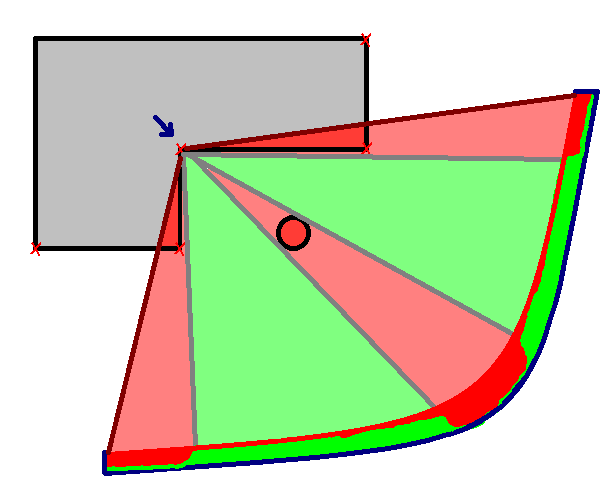
\includegraphics[width=0.45\textwidth]{img/visibilityocclusioncarving}
          \label{fig:visibilitycarving}
 }
 \caption{Graphical example of Visibility-Occlusion Space Carving.}
 \label{fig:vis-occ-carving}
\end{figure}

Assuming the world is occupied by default means that information is needed for every free part of space. In practise, footage often turns out to contain insufficient detected features to recover whole the scene. During initial tests with an implementation of Alg.~\ref{alg:vis-carving} it became clear that reconstructed scenes typically contain a few regions which were free but for which there was simply insufficient positive information (\eg detected features on the background). Here, we present an algorithm that tries to overcome this problem. Regions for which no information is available are marked unknown, while negative information (\ie missing matches) needed to increase the probability of occluded regions. Two versions are presented: the general algorithm, and a slightly altered version for practical reasons.

The presented algorithm starts with a fully unknown world, with some prior probability value for occupancy. Similar to Alg.~\ref{alg:vis-carving}, voxels representing space between camera poses and features. However, both space towards detected and undetected features are affected. To this end, all features are projected onto all image planes. For the features that project inside the window borders of a particular camera (\ie all features that would have been visible if no occluders existed and matching was perfect), we check if they were detected or not. Features that were indeed detected contribute positive information, and so the occupancy probability of space between the particular camera and detected features is \emph{decreased} by a pre-defined constant factor $Pr_{decr}$. Features that did re-project inside the window borders, but were \emph{not} detected, contribute negative information, and so the occupancy probability of space between the camera and undetected features is \emph{increased} by a pre-defined (although potentially different) constant factor $Pr_{incr}$. The process for one interest point is shown in Figure \ref{fig:vis-occ-carving}. The algorithm returns the final probabilistic voxel grid. An occupancy threshold $Thr_{occ}$ can be used to extract binary space partitioning where only voxels with high occupancy probability are set to `occupied'. If desired, a second `free-space' threshold $Thr_{free}$ can be used for visualising voxels that are highly probable to be free. The general version of the algorithm is formalised in Alg.~\ref{alg:vis-occ-carving}.

In practise, occlusion information is often less reliable than (positive) visibility information. Publicly available Structure from Motion solutions often act conservative while creating the visibility lists, and no probabilities are exported (Sect. \ref{implementation}). In the end, claimed visibility of features is very reliable, but claimed invisibility can well be a weak, but correct, match. To solve this balance equality, one could set the positive visibility information factor $Pr_{decr}$ to a high value and set the occlusion information factor $Pr_{incr}$ relatively low. Instead, we propose a modified version of the general algorithm whereby visible features cause a \emph{veto} or absolute vote against occupancy of the space between camera pose and feature. Voxels within this space are set to $Thr_{free}$, which also prevents further increasing of occupancy probability. The modified version is shown in Alg.~\ref{alg:vis-occ-carving-veto}.

Note that all three algorithms require camera models $c$, features $f$, and (binary) visibility lists $v$, which are all provided by standard Structure from Motion techniques. The resolution of the voxel grid $r$ needs to be set too. The two Visibility-Occlusion algorithms also need occupancy prior $Pr_{unknown}$ and probability increasing constant $Pr_{incr}$. The general version needs probability decreasing constant $Pr_{decr}$ too, where the veto version needs the threshold for free space $Thr_{free}$. For visualisation purposes, an occupancy threshold $Thr_{occ}$ can be used too. Appropriate values for these probability and threshold parameters need to be chosen. Parameters $Pr_{unknown}$, $Thr_{free}$ and $Thr_{occ}$ can be kept constant in most cases, and indeed that is the case in the rest of this thesis. However, $Pr_{incr}$ and, if necessary, $Pr_{decr}$, are dependent on the data provided. Relative displacement between subsequent frames, amount of texture in the scene, stability of the features in the dataset, and voxel grid resolution $r$ are all factors that can influence the choice of these parameters. In practise, often a few parameter values can be tried and results can be inspected visually.

{\singlespacing
\begin{algorithm}[!h]
  \centering
  \begin{algorithmic}[1]
    \Function{VisibilityOcclusionSpaceCarving}{$c$, $f$, $v$, $r$, $Pr_{unknown}$, $Pr_{decr}$, $Pr_{incr}$}%, $Thr_{free}$, $Thr_{occ}$}
      \State $G \gets G_{Pr_{unknown}}(r)$ \Comment{Initialise voxel grid $G$ with prior of `unknown' space}
      \ForAll{Camera $c_j$ in $v_{f_i}$}
        \ForAll{Feature $f_i$ in $f$}
          \If{$\mathrm{reprojectsInsideImage}(f_i, c_j)$} \Comment{Get features projecting inside image borders}
            \State $X \gets \mathrm{getVoxelsBetween}(G, c_j, f_i)$ \Comment{Get voxels in between camera and feature}
            \If{$c_j \in v_{f_i}$} \Comment{Feature is visible}
              \ForAll{Voxel $x_i$ in $X$}
                \State $x_i \gets x_i - Pr_{decr}$ \Comment{Thus, decrease occupancy probability}
              \EndFor
            \Else \Comment{Feature was not detected}
              \ForAll{Voxel $x_i$ in $X$}
                \State $x_i \gets x_i + Pr_{incr}$ \Comment{Thus, increase occupancy probability}
              \EndFor
            \EndIf
          \EndIf
        \EndFor
      \EndFor
      \State \Return $H$
    \EndFunction
  \end{algorithmic}
  \caption{Visibility-Occlusion Space Carving - General formulation}
  \label{alg:vis-occ-carving}
\end{algorithm}
}

{\singlespacing
\begin{algorithm}[!h]
  \centering
  \begin{algorithmic}[1]
    \Function{VisibilityOcclusionSpaceCarvingVeto}{$c$, $f$, $v$, $r$, $Pr_{unknown}$, $Pr_{incr}$, $Thr_{free}$}%, $Pr_{decr}, $Thr_{occ}$}
      \State $G \gets G_{Pr_{unknown}}(r)$ \Comment{Initialise voxel grid $G$ with prior of `unknown' space}
      \ForAll{Camera $c_j$ in $v_{f_i}$}
        \ForAll{Feature $f_i$ in $f$}
          \If{$\mathrm{reprojectsInsideImage}(f_i, c_j)$} \Comment{Get features projecting inside image borders}
            \State $X \gets \mathrm{getVoxelsBetween}(G, c_j, f_i)$ \Comment{Get voxels in between camera and feature}
            \If{$c_j \in v_{f_i}$} \Comment{Feature is visible}
              \ForAll{Voxel $x_i$ in $X$}
                \State $x_i \gets Thr_{free}$ \Comment{Thus, use veto and set to free}
              \EndFor
            \Else \Comment{Feature was not detected}
              \ForAll{Voxel $x_i$ in $X$}
                \If{$x_i >= Thr_{free}$} \Comment{Only if veto has not been used ...}
                  \State $x_i \gets x_i + Pr_{incr}$ \Comment{... increase occupancy probability}
                \EndIf
              \EndFor
            \EndIf
          \EndIf
        \EndFor
      \EndFor
      \State \Return $H$
    \EndFunction
  \end{algorithmic}
  \caption{Visibility-Occlusion Space Carving - Veto version}
  \label{alg:vis-occ-carving-veto}
\end{algorithm}
}

% - extending visibility lists
\section{Extending visibility lists}  \label{extend-vis-lists}
Since visibility lists provided by standard SfM tools are often conservative, it is worth exploring possibilities to extend those lists. This is especially true for the proposed Visibility-Occlusion Space Carving algorithms, which rely on missing entries in visibility lists. Early experiments using Alg.~\ref{alg:vis-occ-carving} and Alg.~\ref{alg:vis-occ-carving-veto} indeed showed small uncarved regions caused by incorrectly missing matches. Therefore, a short excursion in extending the visibility lists has been made.

Missing matches are either caused by features being truly occluded, or bad similarity scores by other reasons than invisibility. To discriminate between the two, we project the features, in our case SIFT interest points, into the cameras that did not detect them. Descriptions of the regions around the projected features are extracted, and compared to descriptions of the same points projected onto image planes of the nearest camera that did detect the particular feature. For simplicity, we use patch matching where patches are centred around the projected points, but other descriptors such as SIFT descriptors can be used too. The patches are projections of pieces of geometry with unknown orientation; however, since sequences are used and nearest cameras (in absolute distance) are searched for, it is reasonable to assume that relative orientation with respect to the cameras would not differ too much, and thus projections would not show many differences, if indeed the same geometry is projected. Since we use SIFT features - which do not have a clear size when SfM tools do not export their scale - and we therefore space carve tubes the size of voxels, we chose the size of the patches to be equal to the size of the projected voxel containing the SIFT feature. The descriptors (\ie patches) are compared and thresholded, obtaining possibly new matches. New matches are added to the visibility lists. After extending visibility lists, we can apply one of the Visibility-Occupancy Space Carve algorithms described before. Since the assumption of conservative, thus reliable, visibility lists is now lost and some of the new matches will be incorrect, the veto version is less suited and the general formulation (Alg. \ref{alg:vis-occ-carving}) is preferred.



% (- regularisation)
% TODO: is this working?
% TODO: if so, extend the section?
\section{Regularisation}  \label{regularisation}
The voxel grids returned by the algorithms described all contain voxels that are individual solutions: their occupancy probability or state is independent of their neighbouring voxels' probabilities. To obtain a better global solution we can introduce a prior promoting local smoothness. Together with the proposed algorithms, they form joint voxel-carving algorithms. The voxel grid can be converted to a 3D graph which can be solved by standard min-cut/max-flow graph-cut methods \cite{Boykov2004}. Voxels are thereby represented as nodes and nodes for neighbouring voxels are connected. Nodes have unary costs and pairwise costs. The unary costs $U_i$ for connection with the Sink node are set equal to occupancy probabilities (after truncating to the range $0.0-1.0$), and connection with the Source is set to $1 - U_i$. Pairwise costs could have been based on some photo-consistency comparing appearances of pairs of re-projected voxels, but this would introduce dependencies on appearances again, which were tried to be dropped in the first place. Therefore, pairwise costs are based on differences in occupancy probability weighted with a constant factor, as $P_{i,j} = \gamma * (1 - | U_i - U_j |)$.

